% Created 2021-03-28 Sun 09:10
% Intended LaTeX compiler: pdflatex
\documentclass[12pt,a4paper]{article}
\usepackage[utf8]{inputenc}
\usepackage[T1]{fontenc}
\usepackage{graphicx}
\usepackage{grffile}
\usepackage{longtable}
\usepackage{wrapfig}
\usepackage{rotating}
\usepackage[normalem]{ulem}
\usepackage{amsmath}
\usepackage{textcomp}
\usepackage{amssymb}
\usepackage{capt-of}
\usepackage{hyperref}
\usepackage{minted}
\usepackage{listings}
\usepackage[left=1cm,right=1cm,top=1.5cm, bottom=2cm]{geometry}
\usepackage[utf8]{inputenc}
\usepackage{siunitx}
\usepackage{amsmath}
\usepackage{adjustbox}
\usepackage{tabularx}
\usepackage{booktabs} %Publication quality tables in LaTeX.
\usepackage{pdflscape}
\usepackage[citestyle=authoryear-icomp,bibstyle=authoryear, hyperref=true,backref=true,maxcitenames=3,url=true,backend=biber,natbib=true] {biblatex}
\addbibresource{TFG-Casimir.bib}
\author{casimir}
\date{\today}
\title{Fonones y espectroscopía Raman en semiconductores bidimensionales.}
\hypersetup{
 pdfauthor={casimir},
 pdftitle={Fonones y espectroscopía Raman en semiconductores bidimensionales.},
 pdfkeywords={},
 pdfsubject={},
 pdfcreator={Emacs 27.1 (Org mode 9.4)}, 
 pdflang={English}}
\begin{document}

\maketitle
\tableofcontents

\begin{abstract}
Los materiales bidimensionales (2D) como el grafeno son de gran interés tanto por sus
propiedades físicas exclusivas como por sus aplicaciones potenciales. El estudio de la dinámica de la red cristalina (fonones) de estos materiales es un requisito previo para entender su estabilidad estructural y propiedades térmicas, así como sus propiedades de transporte y ópticas.


Este Trabajo de Fin de Grado consiste en la computación de los modos vibracionales de
materiales semiconductores 2D y su correlación con los observables relevantes para la interpretación de los experimentos de dispersión de luz.

\end{abstract}

\color{blue}
La redacción del TFG todavía se encuentra en una versión muy preliminar, de hecho es más un bloc de notas que lo que espero que sea el TFG final.

Para redactar este trabajo estoy usando \textbf{org-mode} (junto con org-babel, org-ref, \ldots{}): un modo de edición del editor \emph{Emacs}, que, entre otras muchas cosas, permite usar de manera nativa \LaTeX y escribir un mismo fichero tanto el \emph{texto} cómo el \emph{codigo} (en muchos lenguajes, permitiendo también metaprogramación \ldots{}), pudiendo insertar si así se desea la salida de los programas en el mismo documento, y exportat el resultado final a varios formatos (en particular \LaTeX) mostrando u ocultando los bloques con el código en el pdf final.


\normalcolor
\newpage

\section{Lecturas y apuntes de repaso}
\label{sec:orgc6718ff}

Links a los documentos, no es la bibliografía.

La bibliografía va en el fichero TFG-Casimir.bib y la gestiono (así como las referencias) con el paquete org-ref: entre otras cosas añade la referencia en formato bibtex automáticamente al fichero .bib y copia el pdf a mi biblioteca (renombrando el fichero) simplemente arrastrando el pdf al buffer de emacs donde tenemos abierto este fichero. Podemos también insertar manualmente ('M-x crossref-lookup') el título del artículo, lo busca en internet, lo baja si es posible (se pueden añadir fuentes no oficiales), y nos genera la entrada bibtex.

\subsection{Bibliografia basica}
\label{sec:orgf56f4db}
\begin{itemize}
\item \href{Bibliografia/Phonons\_Theory\_and\_Experiments\_I.pdf}{Phonons Theory and Experiments}
\item \href{Bibliografia/wirtz2004.pdf}{wirtz2004}
\item \href{Bibliografia/0802.0912.pdf}{Symmetry constraints on phono dispersion in graphene}
\item \href{Bibliografia/PhysRevB.42.11469.pdf}{Bond softening in monolayer graphite formed on transition-metal carbide surfaces}
\item \href{Bibliografia/kumar2013.pdf}{Phonon dispersions in graphene sheet and single-walled carbon nanotubes}
\item \href{Bibliografia/PFC\_Carlos\_Ventura\_Piazza.pdf}{Matriz de fuerzas, interpretacion, simetrias \ldots{} (pag 29)}
\end{itemize}

\subsection{Repaso de Estado Sólido}
\label{sec:org0b57d41}
\begin{itemize}
\item \href{file:///home/casimir/Documents/Fisica/Biblioteca/Estat\_Solid/Apunts/FES0910\_PortadaxTema\_01.pdf}{Tema 1 de Estado Sólido}
\item \href{file:///home/casimir/Documents/Fisica/Biblioteca/Estat\_Solid/Apunts/FES0910\_Tema02.pdf}{Tema2. Vibraciones atómicas en cristales}
\end{itemize}


\newpage

\section{{\bfseries\sffamily TODO} Introduccion}
\label{sec:org87b1e62}
\color{red}
Por ahora solo algunas ideas que hay que desarrollar.

La idea que tengo es explicar el modelo de  Born y  Von karman (1921), tal y como viene explicado en \cite{brueesch82_phonon}, pagina 4.

Luego explicar que haciendo uso de la aproximación adiabática, \cite{brueesch82_phonon} página 6, podemos, siempre que sea válida tal aproximación -explicar cuando lo es y cuando deja de serlo-, considerar los nucleos ionicos y los elecrones de valencia como constituyentes independientes del sólido, de manera que podemos escribir la energía potencial (o el Hamiltoniano) como una suma de las distintas contribuciones, y que para 

Pasar a describir la aproximación armónica: escribir el potencial, las ecuaciones de movimiento de Lagrange, y pasar de estas ecuaciones de movimiento en el espacio de posiciones al problema de valores propios de la matriz dinámica en el espació de vectores de onda.

Una vez concluida la introducción teórica general, valida para cualquier cristal, escribir el potencial separando el "stretching" y "bendig¨ y escribir la matriz dinámica, teniendo en cuenta que debido a la simetria del cristal la matriz de constantes de fuerza (y su transformada de Fourier, la matriz dinámica), debe cumplir ciertas relaciones (forma de la matriz, elementos nulos, relación entre elementos, \ldots{}), \cite{aizawa90_bond_soften_monol_graph_formed} (en el apendice). Hay que hacer notar que para expresar la matriz de constantes de fuerza en coordenadas cartesianas hay que hacer el correspondiente cambio de coordenadas desde las radiales-transversales.


\normalcolor

Las vibraciones reticulares están regidas por las fuerzas que experimentan los átomos cuando se desplazan de su posición de equilibrio. La primera hipótesis es que cada átomo tiene una posicion de equilibrio en el cristal, y consideraremos que estos átomos vibran con una amplitud pequeña (en comparación con la distancia interatómica) alrededor de su posición de equilibrio, de manera que el sólido se encuentra en estados que corresponden a lo que macroscópicamente se conoce como \emph{la región de comportamiento elástico lineal}, donde se verifica la ley de Hooke.

Podremos por tanto aproximar la energía potencial de interacción por el termino armónico de su desarrolo en serie de potencias del desplazamiento \color{red} desarollar como a partir de la energia potencial del cristal \(\mathcal{U}\), usando una aproximacion armonica, obtenemos la ecuacion secular para los fonones.\normalcolor.

Un fonón es un modo de vibración cuantizado que tiene lugar en una red cristalina. El estudio de los fonones juega un papel muy importante en la física del estado sólido porque los fonones tienen una gran importancia en muchas propiedades físicas de los sólidos. Los fonones son una versión mecano-cuantica de los modos normales de vibración de la mecánica clasica, donde cada parte de la red oscila con la misma frecuencia. Estos modos normales son importantes porque cualquier movimiento vibracional de la red puede describirse como una superposición de modos normales de distinta frecuencia, en este sentido son la base de las vibraciones de la red.



\subsection{{\bfseries\sffamily TODO} Matriz dinámica}
\label{sec:orgcb8aecf}
La matriz dinámica es una cantidad central en la dinámica reticular: las frecuencias de los fonones (vibraciones reticulares cuantificadas) se calculan a partir de los valores propios de la matriz dinámica:

\begin{equation}
\sum_{\alpha\prime}D_{\alpha\alpha\prime}\cdot\vec e_{\alpha\prime}(\vec q)=\omega^{2}\vec e_{\alpha}(\vec q)
\end{equation}   

Por lo tanto, las frecuencias \(\omega\) como función de vector de ondas \(\vec q\) del fonón son solución de la ecuación secular:

\begin{equation}
\det\left|\frac{1}{\sqrt{M_\alpha M_{\alpha\prime}}}D^{ij}_{\alpha\alpha\prime}\left(\vec q\right)-\omega^2\left(\vec q\right)\right| 
\end{equation}

donde \(M_{\alpha}\) es la masa del átomo \(\alpha\) y la matriz dinámica viene definida por:

\begin{equation}
D_{\alpha,\alpha\prime}^{i,j}=\frac{\partial^2 E}{\partial u_{\alpha}^{*i}(\vec q)\partial u_{\alpha\prime}^{j}(\vec q)}
\label{eq:Matriz_Dinámica}
\end{equation}

donde \(u_{\alpha}^{i}\) representa el desplazamiento del átomo \(\alpha\) en la dirección \(i\).

La segunda derivada de la energía de la ecuación \ref{eq:Matriz_Dinámica} corresponde al cambio en la fuerza que actua sobre el átomo \(\alpha\prime\) en la dirección \(j\) cuando se desplaza el átomo \(\alpha\) en la dirección \(i\)

\begin{equation}
D_{\alpha\alpha\prime}^{ij}(\vec q)=\frac{\partial}{\partial u^{*\alpha}_{i}}F^{j}_{\alpha\prime}(\vec q)
\end{equation}

Puesto que el cálculo de los modos de vibración por primeros principios empieza por establecer la geometria del cristal en equilibrio, vamos a comprobar que con los datos proporcionados que el BN monolayer se trata  de un cristal bidimensional de base diatómica, cuya celda unidad viene dada por (datos proporcionados):

\begin{equation}
\vec a_1=a(1,0);\qquad\vec a_2=a\left(-\frac{1}{2},\frac{\sqrt{3}}{2}\right)
\end{equation}


\begin{minted}[]{python}
import numpy as np
from  numpy  import array, sqrt, sort, vdot, pi, arccos
from numpy.linalg import norm
import pandas as pd
import matplotlib
from matplotlib import pyplot as plt

a=1 
a_1=np.array([a,0])
a_2=np.array([-a/2,sqrt(3)*a/2])
\end{minted}

Podemos comprobar que efectivamente se trata de una celdilla hexagonal, pues los dos vectores base forman un angulo de \(\SI{2\pi/3}{\radian}\)


Numeraremos las celdillas unidad con un índice vectorial \(\vec l=\left( l_1, l_2\right)\), notemos que aunque es habitual representar la celdilla con un indice entero \(n\) es más sencillo y facilita los cálculos (así como determinar a que celdilla no referimos) el uso de un índice vectorial. Las posiciones de los nudos son \(\vec R_{\vec l}=l_1\vec{a}_1+l_2\vec{a}_2\).

Visualizamos una región de la red hexagonal, con los correspondientes nudos (que no átomos), así como la correspondiente celda unidad,

\vspace{0.5cm}
\begin{minipage}{0.55\textwidth}
\begin{minted}[]{python}
def R_l(l_1,l_2):
 return l_1*a_1+l_2*a_2 

reddenudos=array([R_l(l_1,l_2) for l_1 in range(-3, 4)
  for l_2 in range(-3,4)])

x = reddenudos[:,0]
y = reddenudos[:,1]
plt.plot(x,y,"o")
ax = plt.axes()
ax.arrow(R_l(0,0)[0],R_l(0,0)[1],
	 R_l(1,0)[0],R_l(1,0)[1])
ax.arrow(R_l(0,0)[0],R_l(0,0)[1],
	 R_l(0,1)[0],R_l(0,1)[1])
plt.savefig("Graficas/Reddenudos.jpg")
plt.close()
\end{minted}

\end{minipage}\begin{minipage}{0.55\textwidth}
\begin{center}
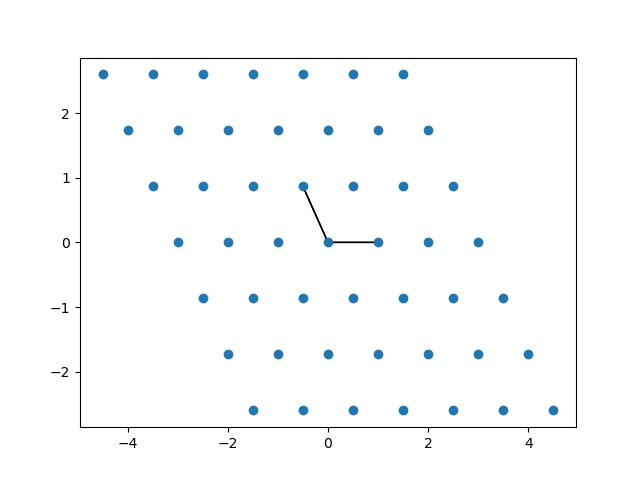
\includegraphics[width=8cm]{Graficas/Reddenudos.jpg}
\end{center}
\end{minipage}

\vspace{0.5cm}
\color{red}
Hacer figuras de la red reciproca, primera zona de Brillouin (y puntos especiales, Gamma, K, K', M).
\normalcolor

\vspace{0.7cm}
Para calcular los modos de vibración por primeros principios debemos determinar primero las posiciones atómicas de equilibrio  en la celda unidad \textbf{\textbf{nota: proporcionadas como datos}}

Los átomos estan situados en:

\begin{equation}
\begin{aligned}
\vec R_B&=\frac{1}{3}\vec{a_1}+2\vec{a_2}\\
\vec R_N&=\frac{2}{3}\vec{a_1}+\frac{1}{3}\vec{a_2}
\end{aligned}
\end{equation}

\begin{minted}[]{python}
R_B=1/3*a_1+2/3*a_2
R_N=2/3*a_1+1/3*a_2
\end{minted}

Las posiciones de equilibrio de los átomos de la base respecto de su nudo son \(\vec{R}_\alpha^0\) , con \(\alpha=1,2\), puesto que la base tiene 2 átomos, el \(1\) hará referencia a los átomos de \(B\) y \(2\) a los de átomos de \(N\) (notemos que aunque los átomos fuesen idénticos tendriamos que especificar a que átomo de la base nos referimos, puesto que no ocupan posiciones equivalentes).


Las posiciones de equilibrio de los átomos: \(\vec R_{\alpha,\vec l}=\vec{R}_{\vec{l}} + \vec R_\alpha^0\)  así como los desplazamientos atómicos: \(\vec u_{\alpha,\vec l}\) quedarán por tanto identificados por medio de dos índices.

Pasamor ahora a representar la red de átomos:

\begin{minipage}{0.55\textwidth}
\begin{minted}[]{python}
#Posiciones de equilibrio de los átomos

def R_alpha_l(alpha,l_1,l_2):
  if alpha == 1:
    return l_1*a_1+l_2*a_2+R_B

  elif alpha == 2:
    return l_1*a_1+l_2*a_2+R_N

  else:
    print("Error, alpha solo puede ser 1 o 2 ")

AtomosB=array([R_alpha_l(1,l_1,l_2) for l_1 in range(-4, 5)
	       for l_2 in range(-4,5)])

AtomosN=array([R_alpha_l(2,l_1,l_2) for l_1 in range(-4, 5)
	       for l_2 in range(-4,5)])

xB = AtomosB[:,0]
yB = AtomosB[:,1]
plt.plot(xB,yB,"o",color="red")

xN = AtomosN[:,0]
yN = AtomosN[:,1]
plt.plot(xN,yN,"o",color="blue")

plt.savefig("Graficas/Reddeatomos.jpg")
plt.close()
\end{minted}

\end{minipage}\begin{minipage}{0.6\textwidth}
\begin{center}
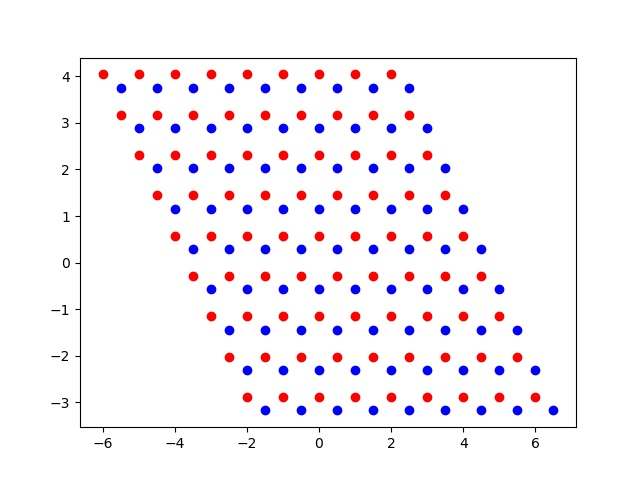
\includegraphics[width=6 cm]{Graficas/Reddeatomos.jpg}
\end{center}
\end{minipage}

\vspace{0.5cm}
Las dimensiones del cristal son \(L_1=N_1 a_1\) y \(L_2=N_2 a_2\), donde \(N_i\) (\(i=1,2\)) es el número de celdillas en la dirección \(\vec a_i\). El cristal tiene tiene \(N=N_1N_2\) celdillas unidad primitivas y \(2N\) átomos.


\textbf{La idea básica es que si la base tiene \(r\) átomos entonces debemos plantear y resolver las ecuaciones de movimiento de los \(r\) átomos de la base de la celdilla \(\vec 0\)}, por lo tanto en el caso que estamos estudiando debemos resolver 2 ecuaciones vectoriales de movimiento: una para el átomo de \(B\) y la otra para el de \(N\).

\color{red} Falta reescribir completamente y ampliar mucho la introducción teórica


Notar que aunque el cristal sea bi-dimensional, los átomos de este pueden vibrar en las 3 direcciones espaciales.

Explicar que podemos tratar por un lado las vibraciones en el plano del cristal y por otro las vibraciones perpendiculares a este, ya que se trata de vibraciones completamente desacopladas.

Que la  ecuación secular tiene \(3 N_\nu=6\) soluciones que describen las \(6\) ramas de la relación de dispersión, es decir, las \(6\) frecuencias características de los \(6\) modos normales de vibración de vector de onda \(\vec q\). Se cumple que el número total de modos normales de vibración coincide con el triple del número total de átomos, es decir, \textit{con el de grados de libertad de movimiento de los átomos}

Puesto que la energia potencial es una funcion cuadratica \cite{falkovsky08_symmet_const_phonon_disper_graph}

\normalcolor

\newpage
\section{{\bfseries\sffamily TODO} Desarrollo del trabajo}
\label{sec:org5c244cf}

\subsection{Clasificación de los vecinos}
\label{sec:org878cecf}

Puesto que debemos determinar cuales son las posiciones de equilibrio de los átomos más cercanos a los átomos de la celda \(\vec 0\) antes que nada genero un array con los datos que voy a necesitar, ordenando las filas de manera creciente a la distancia a cada uno de los 2 átomos de la celda  \(l=\vec 0\) hasta los cuartos vecinos, y guardando el array con la información como un DataFrame de pandas, que facilita mucho la manipulación de los datos.



\begin{minted}[]{python}
from sympy import *
import pandas as pd

## Parametros de la red, de la celdilla y del cristal
a=Symbol('a', real=True, positive=True)
q_x=Symbol('q_x', real=True);  q_y=Symbol('q_y', real=True)
q=Matrix([q_x,q_y])
a_1=Matrix([a,0]); a_2=Rational(1,2)*Matrix([-a,sqrt(3)*a])
R_B=Rational(1,3)*a_1+Rational(2,3)*a_2; R_N=Rational(2,3)*a_1+Rational(1,3)*a_2

## Masas de los átomos, frecuencia, ...
M_B, M_N, omega=symbols("M_B, M_N, omega") #masa de los átomos de Boro y N.
def masa(alpha):
  if alpha == 1:
    return M_B

  elif alpha == 2:
    return M_N

  else:
    print("Error, alpha sólo puede se 1 o 2")


## Vector R_l (vector de traslación primitivo)
def R_l(l_1,l_2):
  return l_1*a_1+l_2*a_2

## Vector de posición de los átomos del cristal (en equilibrio)
def R_alpha_l(alpha,l_1,l_2):
  if alpha == 1:
    return l_1*a_1+l_2*a_2+R_B

  elif alpha == 2:
    return l_1*a_1+l_2*a_2+R_N

  else:
    print("Error, alpha solo puede ser 1 o 2 ")

## Vector unitario que une uno de los átomos en la celdilla 0 con el átomo considerado
def R_hat(alphaprima,alpha,l_1,l_2):
  if (R_alpha_l(alpha,l_1,l_2)-R_alpha_l(alphaprima,0,0)).norm()>0:
    return (R_alpha_l(alpha,l_1,l_2)-R_alpha_l(alphaprima,0,0))/(R_alpha_l(alpha,l_1,l_2)
						     -R_alpha_l(alphaprima,0,0)).norm()

  else:
    return (R_alpha_l(alpha,l_1,l_2)-R_alpha_l(alphaprima,0,0))

def fase(l_1,l_2):
  return exp(I*q.dot(R_l(l_1,l_2)))

## Finalmente construyo un DataFrame de pandas con la información necesaria para
## identificar a los primeros, segundos, ... vecinos, según su distancia a cada uno
## de los átomos de la celdilla unidad
def propiedades_atomos(l_1, l_2):
  return [(k, m, i, j,  R_hat(k,m,i,j),fase(i,j), (R_alpha_l(m,i,j)-R_alpha_l(k,0,0)).norm()/a)
      for k in [1,2] for m in [1,2]  for i in range(-l_1,l_1+1) for j in range(-l_2,l_2+1)]

columnas = [r"$\alpha\prime$",r"$\alpha$",r"$l_1$", r"$l_2$",r"$\hat R_{\nu\prime,\nu,\vec l}$",
 'Fase','Distancia']

def Atomos(l_1, l_2):
  return pd.DataFrame(propiedades_atomos(l_1,l_2),columns=columnas).sort_values(
       ['Distancia',r"$\alpha\prime$"], ascending=[True, True])
## Mostramos el dataframe como una tabla en formato \LaTeX.
Atomos(2,2).head(26).to_latex(escape=False,float_format="{:0.4f}".format,index=False)
\end{minted}

\begin{tabular}{rrrrlll}
\toprule
 $\alpha\prime$ &  $\alpha$ &  $l_1$ &  $l_2$ & $\hat R_{\nu\prime,\nu,\vec l}$ &                                   Fase &    Distancia \\
\midrule
              1 &         1 &      0 &      0 &                          [0, 0] &                                      1 &            0 \\
              2 &         2 &      0 &      0 &                          [0, 0] &                                      1 &            0 \\
              1 &         2 &     -1 &      0 &              [-sqrt(3)/2, -1/2] &                          exp(-I*a*q_x) &    sqrt(3)/3 \\
              1 &         2 &      0 &      0 &               [sqrt(3)/2, -1/2] &                                      1 &    sqrt(3)/3 \\
              1 &         2 &      0 &      1 &                          [0, 1] &    exp(I*(-a*q_x/2 + sqrt(3)*a*q_y/2)) &    sqrt(3)/3 \\
              2 &         1 &      0 &     -1 &                         [0, -1] &     exp(I*(a*q_x/2 - sqrt(3)*a*q_y/2)) &    sqrt(3)/3 \\
              2 &         1 &      0 &      0 &               [-sqrt(3)/2, 1/2] &                                      1 &    sqrt(3)/3 \\
              2 &         1 &      1 &      0 &                [sqrt(3)/2, 1/2] &                           exp(I*a*q_x) &    sqrt(3)/3 \\
              1 &         1 &     -1 &     -1 &              [-1/2, -sqrt(3)/2] &    exp(I*(-a*q_x/2 - sqrt(3)*a*q_y/2)) &            1 \\
              1 &         1 &     -1 &      0 &                         [-1, 0] &                          exp(-I*a*q_x) &            1 \\
              1 &         1 &      0 &     -1 &               [1/2, -sqrt(3)/2] &     exp(I*(a*q_x/2 - sqrt(3)*a*q_y/2)) &            1 \\
              1 &         1 &      0 &      1 &               [-1/2, sqrt(3)/2] &    exp(I*(-a*q_x/2 + sqrt(3)*a*q_y/2)) &            1 \\
              1 &         1 &      1 &      0 &                          [1, 0] &                           exp(I*a*q_x) &            1 \\
              1 &         1 &      1 &      1 &                [1/2, sqrt(3)/2] &     exp(I*(a*q_x/2 + sqrt(3)*a*q_y/2)) &            1 \\
              2 &         2 &     -1 &     -1 &              [-1/2, -sqrt(3)/2] &    exp(I*(-a*q_x/2 - sqrt(3)*a*q_y/2)) &            1 \\
              2 &         2 &     -1 &      0 &                         [-1, 0] &                          exp(-I*a*q_x) &            1 \\
              2 &         2 &      0 &     -1 &               [1/2, -sqrt(3)/2] &     exp(I*(a*q_x/2 - sqrt(3)*a*q_y/2)) &            1 \\
              2 &         2 &      0 &      1 &               [-1/2, sqrt(3)/2] &    exp(I*(-a*q_x/2 + sqrt(3)*a*q_y/2)) &            1 \\
              2 &         2 &      1 &      0 &                          [1, 0] &                           exp(I*a*q_x) &            1 \\
              2 &         2 &      1 &      1 &                [1/2, sqrt(3)/2] &     exp(I*(a*q_x/2 + sqrt(3)*a*q_y/2)) &            1 \\
              1 &         2 &     -1 &     -1 &                         [0, -1] &    exp(I*(-a*q_x/2 - sqrt(3)*a*q_y/2)) &  2*sqrt(3)/3 \\
              1 &         2 &     -1 &      1 &               [-sqrt(3)/2, 1/2] &  exp(I*(-3*a*q_x/2 + sqrt(3)*a*q_y/2)) &  2*sqrt(3)/3 \\
              1 &         2 &      1 &      1 &                [sqrt(3)/2, 1/2] &     exp(I*(a*q_x/2 + sqrt(3)*a*q_y/2)) &  2*sqrt(3)/3 \\
              2 &         1 &     -1 &     -1 &              [-sqrt(3)/2, -1/2] &    exp(I*(-a*q_x/2 - sqrt(3)*a*q_y/2)) &  2*sqrt(3)/3 \\
              2 &         1 &      1 &     -1 &               [sqrt(3)/2, -1/2] &   exp(I*(3*a*q_x/2 - sqrt(3)*a*q_y/2)) &  2*sqrt(3)/3 \\
              2 &         1 &      1 &      1 &                          [0, 1] &     exp(I*(a*q_x/2 + sqrt(3)*a*q_y/2)) &  2*sqrt(3)/3 \\
\bottomrule
\end{tabular}






\newpage

\subsection{Matriz de constantes de fuerza y matriz dinámica}
\label{sec:org413eae3}

A parte de identificar los primeros, segundos, \ldots{} vecinos, necesitamos conocer la matriz de constantes de fuerza que corresponde a la interacción de cada átomo de la celdilla unidad con su n-esimo vecino.

Vamos a suponer (por simplificar) que un desplazamiento longitudinal (radial, que estará contenido en el plano del cristal) o transversal (tangencial, sea en el plano o perpendicular al plano) solo genera una fuerza radial o transversal.

\color{red}
Dibujar un esquema tipo
\begin{center}
\includegraphics[width=6 cm]{Graficas/Esquema_Matriz_Constantes_de_fuerza.png}
\end{center}
\normalcolor
\subsubsection{Primeros vecinos}
\label{sec:org5dcb10a}
Para hacer más explicito el método que he seguido se muestra las matriz de constantes de fuerza para los primeros vecinos del boro 

\color{red} 
Dibujar el boro, y sus vecinos 
\normalcolor

\begin{minted}[]{python}
PrimerosVecinosBoro= Atomos(1,1)[(Atomos(1,1)['Distancia']<0.9) &\
(Atomos(1,1)['Distancia']>0) & (Atomos(1,1)[r"$\alpha\prime$"]==1)]
PrimerosVecinosBoro.to_latex(escape=False)
\end{minted}

\begin{tabular}{lrrrrlll}
\toprule
{} &  $\alpha\prime$ &  $\alpha$ &  $l_1$ &  $l_2$ & $\hat R_{\nu\prime,\nu,\vec l}$ &                                 Fase &  Distancia \\
\midrule
10 &               1 &         2 &     -1 &      0 &              [-sqrt(3)/2, -1/2] &                        exp(-I*a*q_x) &  sqrt(3)/3 \\
13 &               1 &         2 &      0 &      0 &               [sqrt(3)/2, -1/2] &                                    1 &  sqrt(3)/3 \\
14 &               1 &         2 &      0 &      1 &                          [0, 1] &  exp(I*(-a*q_x/2 + sqrt(3)*a*q_y/2)) &  sqrt(3)/3 \\
\bottomrule
\end{tabular}

Podemos observar que para el átomo de nitrogeno de la celdilla \(\vec l = (0,1)\) la correspondiente matriz de constantes de fuerza puede escribirse (en coordenadas cartesianas) como:

\begin{minted}[]{python}
phi_1r__BN,phi_1ti__BN,phi_1to__BN=symbols('phi_1r__BN,phi_1ti__BN,phi_1to__BN')

Phi_10__BN=Matrix([[phi_1ti__BN,0,0],[0,phi_1r__BN,0],[0,0,phi_1to__BN]])
print(r"\begin{equation}D_{1,(0,1)}^{BN}=", latex(Phi_10__BN),r"\end{equation}")
\end{minted}

\begin{equation}
D_{1,(0,1)}^{BN}= \left[\begin{matrix}\phi^{BN}_{1ti} & 0 & 0\\0 & \phi^{BN}_{1r} & 0\\0 & 0 & \phi^{BN}_{1to}\end{matrix}\right]
\end{equation}

\vspace{0.7cm}



donde \(\phi_r\) hace referencia a la constante de fuerza en la dirección radial (\emph{bond stretching}) y \(\phi_{ti}\) y \(\phi_{to}\) a las constantes de fuerza en dirección tangencial (\emph{bond bending}) dentro y fuera de plano, respectivamente.

Puesto que los otros dos primeros vecinos del boro son átomos exactamente iguales que este, y a la misma distancia, podemos calcular sus respectivas matrices de fuerza simplemente rotando esta matriz:
\begin{equation}
\label{eq:2}
\Phi^1_{\vec l}=U_{\vec l}^{-1}\Phi^1U_{\vec l}
\end{equation}

Donde \(U_{\vec l}\) es la matriz de rotación para llevar el átomo de nitrogeno que esta en la celdilla \(\vec l=(0, 1)\) a la posición que ocupan cada uno de los otros primeros vecinos en sus respectivas celdillas.

Por lo tanto tenemos que para el átomo situado en \(\vec l=(-1,0)\)
\begin{minted}[]{python}
phi_1r__BN,phi_1ti__BN,phi_1to__BN=symbols('phi_1r__BN,phi_1ti__BN,phi_1to__BN')

Phi_10__BN=Matrix([[phi_1ti__BN,0,0],[0,phi_1r__BN,0],[0,0,phi_1to__BN]])

def U(theta):
  return Matrix([[cos(theta),sin(theta),0], [-sin(theta), cos(theta),0],[0,0,1]])

# Para el átomo que ocupa la posición l_1=-1,0
def Phi_1l__BN(theta):
  return U(-theta)*Phi_10__BN*U(theta)

print_latex(Matrix([Phi_1l__BN(2*pi/3)[i,j].factor() for j in range(3) for i in range(3)]).reshape(3,3))
\end{minted}

\begin{equation}
\label{eq:3}
\left[\begin{matrix}\frac{3 \phi^{BN}_{1r} + \phi^{BN}_{1ti}}{4} & \frac{\sqrt{3} \left(\phi^{BN}_{1r} - \phi^{BN}_{1ti}\right)}{4} & 0\\\frac{\sqrt{3} \left(\phi^{BN}_{1r} - \phi^{BN}_{1ti}\right)}{4} & \frac{\phi^{BN}_{1r} + 3 \phi^{BN}_{1ti}}{4} & 0\\0 & 0 & \phi^{BN}_{1to}\end{matrix}\right]
\end{equation}

\begin{equation}
\label{eq:11}
\left[\begin{matrix}\frac{3 \phi^{BN}_{1r}}{4} + \frac{\phi^{BN}_{1ti}}{4} & \frac{\sqrt{3} \phi^{BN}_{1r}}{4} - \frac{\sqrt{3} \phi^{BN}_{1ti}}{4} & 0\\\frac{\sqrt{3} \phi^{BN}_{1r}}{4} - \frac{\sqrt{3} \phi^{BN}_{1ti}}{4} & \frac{\phi^{BN}_{1r}}{4} + \frac{3 \phi^{BN}_{1ti}}{4} & 0\\0 & 0 & \phi^{BN}_{1to}\end{matrix}\right]
\end{equation}

Mientras que para el átomo situado en \(\vec l= (0,0)\) la matriz de constantes de fuerza es:

\begin{minted}[]{python}
print_latex(Phi_1l__BN(-2*pi/3))
\end{minted}

\begin{equation}
 \left[\begin{matrix}\frac{3 \phi^{BN}_{1r}}{4} + \frac{\phi^{BN}_{1ti}}{4} & - \frac{\sqrt{3} \phi^{BN}_{1r}}{4} + \frac{\sqrt{3} \phi^{BN}_{1ti}}{4} & 0\\- \frac{\sqrt{3} \phi^{BN}_{1r}}{4} + \frac{\sqrt{3} \phi^{BN}_{1ti}}{4} & \frac{\phi^{BN}_{1r}}{4} + \frac{3 \phi^{BN}_{1ti}}{4} & 0\\0 & 0 & \phi^{BN}_{1to}\end{matrix}\right]
\end{equation}

\newpage
\eject \pdfpagewidth=297mm \pdfpageheight=300mm

Por lo tanto, la contribución a matriz dinámica que tenemos por parte de la interacción de estos primeros vecinos es:

\begin{minted}[]{python}
Phi_1__BN=Phi_10__BN*fase(0,1)+Phi_1l__BN(2*pi/3)*fase(-1,0)+Phi_1l__BN(-2*pi/3)*fase(0,0)
#Phi_1__BN=Matrix([Phi_1__BN[i,j].rewrite(cos).simplify() for i in range(3) for j in range(3)]).reshape(3,3)
\end{minted}

\begin{equation}
\left[\begin{matrix}\frac{3 \phi^{BN}_{1r}}{4} + \frac{\phi^{BN}_{1ti}}{4} + \phi^{BN}_{1ti} e^{- \frac{i a \left(q_{x} - \sqrt{3} q_{y}\right)}{2}} + \frac{\left(3 \phi^{BN}_{1r} + \phi^{BN}_{1ti}\right) e^{- i a q_{x}}}{4} & \frac{\sqrt{3} \left(- \phi^{BN}_{1r} + \phi^{BN}_{1ti} - \left(- \phi^{BN}_{1r} + \phi^{BN}_{1ti}\right) e^{- i a q_{x}}\right)}{4} & 0\\\frac{\sqrt{3} \left(- \phi^{BN}_{1r} + \phi^{BN}_{1ti} - \left(- \phi^{BN}_{1r} + \phi^{BN}_{1ti}\right) e^{- i a q_{x}}\right)}{4} & \frac{\phi^{BN}_{1r}}{4} + \phi^{BN}_{1r} e^{- \frac{i a \left(q_{x} - \sqrt{3} q_{y}\right)}{2}} + \frac{3 \phi^{BN}_{1ti}}{4} + \frac{\left(\phi^{BN}_{1r} + 3 \phi^{BN}_{1ti}\right) e^{- i a q_{x}}}{4} & 0\\0 & 0 & \phi^{BN}_{1to} \left(1 + e^{- \frac{i a \left(q_{x} - \sqrt{3} q_{y}\right)}{2}} + e^{- i a q_{x}}\right)\end{matrix}\right]
\end{equation}

De manera análoga, para los primeros vecinos del átomo de nitrogeno

\begin{minted}[]{python}
PrimerosVecinosNitrogeno= Atomos(1,1)[(Atomos(1,1)['Distancia']<0.9) & \
(Atomos(1,1)['Distancia']>0) & (Atomos(1,1)[r"$\alpha\prime$"]==2)]
PrimerosVecinosNitrogeno.to_latex(escape=False)
\end{minted}

\begin{tabular}{lrrrrlll}
\toprule
{} &  $\alpha\prime$ &  $\alpha$ &  $l_1$ &  $l_2$ & $\hat R_{\nu\prime,\nu,\vec l}$ &                                Fase &  Distancia \\
\midrule
21 &               2 &         1 &      0 &     -1 &                         [0, -1] &  exp(I*(a*q_x/2 - sqrt(3)*a*q_y/2)) &  sqrt(3)/3 \\
22 &               2 &         1 &      0 &      0 &               [-sqrt(3)/2, 1/2] &                                   1 &  sqrt(3)/3 \\
25 &               2 &         1 &      1 &      0 &                [sqrt(3)/2, 1/2] &                        exp(I*a*q_x) &  sqrt(3)/3 \\
\bottomrule
\end{tabular}

\vspace{0.5cm}

Por simetría, la matriz de constantes de fuerza para la interacción entre el átomo de nitrogeno y su primer vecino situado en \(\vec l= (0,-1)\) es igual a la que hemos visto antes para el átomo de boro en la celdilla \(\vec l= (0,0)\) y su primer vecino (un átomo de nitrogeno) en la celdilla \(\vec l= (0,1)\):

Y por lo tanto, la contribución a matriz dinámica que tenemos por parte de la interacción de estos primeros vecinos es:

\begin{minted}[]{python}
Phi_10__NB=Phi_10__BN
def Phi_1l__NB(theta):
  return U(-theta)*Phi_10__NB*U(theta)

Phi_1__NB=Phi_10__NB*fase(0,-1)+Phi_1l__NB(2*pi/3)*fase(1,0)+Phi_1l__NB(-2*pi/3)*fase(0,0)
#Phi_1__NB=(Matrix([Phi_1__NB[i,j].rewrite(cos).simplify() for i in range(3) for j in range(3)]).reshape(3,3))
\end{minted}

\begin{equation}
\left[\begin{matrix}\frac{3 \phi^{BN}_{1r}}{4} + \phi^{BN}_{1ti} e^{\frac{i a \left(q_{x} - \sqrt{3} q_{y}\right)}{2}} + \frac{\phi^{BN}_{1ti}}{4} + \frac{\left(3 \phi^{BN}_{1r} + \phi^{BN}_{1ti}\right) e^{i a q_{x}}}{4} & \frac{\sqrt{3} \left(- \phi^{BN}_{1r} + \phi^{BN}_{1ti} + \left(\phi^{BN}_{1r} - \phi^{BN}_{1ti}\right) e^{i a q_{x}}\right)}{4} & 0\\\frac{\sqrt{3} \left(- \phi^{BN}_{1r} + \phi^{BN}_{1ti} + \left(\phi^{BN}_{1r} - \phi^{BN}_{1ti}\right) e^{i a q_{x}}\right)}{4} & \phi^{BN}_{1r} e^{\frac{i a \left(q_{x} - \sqrt{3} q_{y}\right)}{2}} + \frac{\phi^{BN}_{1r}}{4} + \frac{3 \phi^{BN}_{1ti}}{4} + \frac{\left(\phi^{BN}_{1r} + 3 \phi^{BN}_{1ti}\right) e^{i a q_{x}}}{4} & 0\\0 & 0 & \phi^{BN}_{1to} \left(e^{i a q_{x}} + e^{\frac{i a \left(q_{x} - \sqrt{3} q_{y}\right)}{2}} + 1\right)\end{matrix}\right]
\end{equation}

Debemos hacer notar que \emph{como la energía potencial es una función cuadrática de los desplazamientos atómicos \(u^B_i(\vec R_{\vec l})\) \(u^N_i(\vec R_{\vec l})\) la matriz de constantes de fuerza tiene la forma \(\phi_{ij}^{BN}(\vec R_{\vec l})=\phi_{ji}^{NB}(-\vec R_{\vec l})\), y su transformada de Fourier, es decir, la matriz dinámica, es una matriz Hermítica} (\cite{falkovsky08_symmet_const_phonon_disper_graph}), y también que las vibraciones fuera de plano, en la dirección \(z\) no estan acopladas a las interplanares.

\newpage
\eject \pdfpagewidth=210mm \pdfpageheight=297mm

\subsubsection{Segundos vecinos y terceros vecinos}
\label{sec:orgca2624e}

Calculamos ahora las contribuciones a la matriz dinámica de los segundos y terceros vecinos.

\begin{minted}[]{python}
SegundosVecinosBoro= Atomos(1,1)[(Atomos(1,1)['Distancia']<1.1) &\
(Atomos(1,1)['Distancia']>0.9) & (Atomos(1,1)[r"$\alpha\prime$"]==1)]
##SegundosVecinosBoro.to_latex(escape=False)
\end{minted}

Tenemos \(6\) segundos vecinos para cada uno de los dos átomos de la celdilla unidad y en este caso las interacciones son entre el mismo tipo de átomo. Fijandonos en el átomo de boro situado en la celdilla \(\vec l=(1,0)\) podemos escribir la matriz de constantes de fuerza como:

\begin{equation}
\Phi_{2,(1,0)}^{BB}=\begin{pmatrix}
\phi_{2r}^{(BB)} & 0 & 0 \\
0 & \phi_{2ti}^{(BB)} & 0 \\
 0 & 0  & \phi_{2to}^{(BB)}
\end{pmatrix}
\end{equation} 

mientras que para el atómo de nitrogeno la matriz de constantes de fuerza para el átomo situado en la celdilla \(\vec l =(1,0)\) es:

\begin{equation}
\Phi_{2,(1,0)}^{NN}=\begin{pmatrix}
\phi_{2r}^{(NN)} & 0 & 0 \\
0 & \phi_{2ti}^{(NN)} & 0 \\
 0 & 0  & \phi_{2to}^{(NN)}
\end{pmatrix}
\end{equation} 

y por tanto, la contribución a la matriz dinámica debida a estas interacciones será:

\begin{minted}[]{python}
phi_2r__BB,phi_2ti__BB,phi_2to__BB=symbols('phi_2r__BB,phi_2ti__BB,phi_2to__BB')

 # Para el átomo que ocupa la posición l=1,0
Phi_20__BB=Matrix([[phi_2ti__BB,0,0],[0,phi_2r__BB,0],[0,0,phi_2to__BB]])

def Phi_2l__BB(theta):
  return U(-theta)*Phi_20__BB*U(theta)

Phi_2__BB=Phi_20__BB*fase(1,0)+Phi_2l__BB(pi/3)*fase(1,1)+Phi_2l__BB(-pi/3)*fase(0,-1) \
+Phi_2l__BB(pi)*fase(-1,0)+Phi_2l__BB(2*pi/3)*fase(0,1)+ Phi_2l__BB(-2*pi/3)*fase(-1,-1)

#Phi_2_BB=Matrix([Phi_2__BB[i,j].rewrite(cos).simplify() for i in range(3) \
# for j in range(3)]).reshape(3,3)

SegundosVecinosNitrogeno= Atomos(1,1)[(Atomos(1,1)['Distancia']<1.1) &\
(Atomos(1,1)['Distancia']>0.9) & (Atomos(1,1)[r"$\alpha\prime$"]==2)]
#SegundosVecinosNitrogeno.to_latex(escape=False)

phi_2r__NN,phi_2ti__NN,phi_2to__NN=symbols('phi_2r__NN,phi_2ti__NN,phi_2to__NN')

Phi_20__NN=Matrix([[phi_2ti__NN,0,0],[0,phi_2r__NN,0],[0,0,phi_2to__NN]])

# Para el átomo que ocupa la posición l=1,0
def Phi_2l__NN(theta):
  return U(-theta)*Phi_20__NN*U(theta)

Phi_2__NN=Phi_20__NN*fase(1,0)+Phi_2l__NN(pi/3)*fase(1,1)+Phi_2l__NN(-pi/3)*fase(0,-1) \
      +Phi_2l__NN(pi)*fase(-1,0)+Phi_2l__NN(2*pi/3)*fase(0,1)+Phi_2l__NN(-2*pi/3)*fase(-1,-1)
#Phi_2__NN=Matrix([Phi_2__NN[i,j].rewrite(cos).simplify() for i in range(3) for j in range(3)]).reshape(3,3)

\end{minted}

\newpage
\eject \pdfpagewidth=360mm \pdfpageheight=210mm

\begin{equation}
\left[\begin{matrix}3 \phi^{BB}_{2r} \cos{\left(\frac{a q_{x}}{2} \right)} \cos{\left(\frac{\sqrt{3} a q_{y}}{2} \right)} + \phi^{BB}_{2ti} \cos{\left(\frac{a q_{x}}{2} \right)} \cos{\left(\frac{\sqrt{3} a q_{y}}{2} \right)} + 2 \phi^{BB}_{2ti} \cos{\left(a q_{x} \right)} & \sqrt{3} \left(\phi^{BB}_{2r} - \phi^{BB}_{2ti}\right) \sin{\left(\frac{a q_{x}}{2} \right)} \sin{\left(\frac{\sqrt{3} a q_{y}}{2} \right)} & 0\\\sqrt{3} \left(\phi^{BB}_{2r} - \phi^{BB}_{2ti}\right) \sin{\left(\frac{a q_{x}}{2} \right)} \sin{\left(\frac{\sqrt{3} a q_{y}}{2} \right)} & \phi^{BB}_{2r} \cos{\left(\frac{a q_{x}}{2} \right)} \cos{\left(\frac{\sqrt{3} a q_{y}}{2} \right)} + 2 \phi^{BB}_{2r} \cos{\left(a q_{x} \right)} + 3 \phi^{BB}_{2ti} \cos{\left(\frac{a q_{x}}{2} \right)} \cos{\left(\frac{\sqrt{3} a q_{y}}{2} \right)} & 0\\0 & 0 & 2 \phi^{BB}_{2to} \left(2 \cos{\left(\frac{a q_{x}}{2} \right)} \cos{\left(\frac{\sqrt{3} a q_{y}}{2} \right)} + \cos{\left(a q_{x} \right)}\right)\end{matrix}\right]
\end{equation}

\vspace{1cm}


\begin{equation}
\label{eq:4}
\left[\begin{matrix}3 \phi^{NN}_{2r} \cos{\left(\frac{a q_{x}}{2} \right)} \cos{\left(\frac{\sqrt{3} a q_{y}}{2} \right)} + \phi^{NN}_{2ti} \cos{\left(\frac{a q_{x}}{2} \right)} \cos{\left(\frac{\sqrt{3} a q_{y}}{2} \right)} + 2 \phi^{NN}_{2ti} \cos{\left(a q_{x} \right)} & \sqrt{3} \left(\phi^{NN}_{2r} - \phi^{NN}_{2ti}\right) \sin{\left(\frac{a q_{x}}{2} \right)} \sin{\left(\frac{\sqrt{3} a q_{y}}{2} \right)} & 0\\\sqrt{3} \left(\phi^{NN}_{2r} - \phi^{NN}_{2ti}\right) \sin{\left(\frac{a q_{x}}{2} \right)} \sin{\left(\frac{\sqrt{3} a q_{y}}{2} \right)} & \phi^{NN}_{2r} \cos{\left(\frac{a q_{x}}{2} \right)} \cos{\left(\frac{\sqrt{3} a q_{y}}{2} \right)} + 2 \phi^{NN}_{2r} \cos{\left(a q_{x} \right)} + 3 \phi^{NN}_{2ti} \cos{\left(\frac{a q_{x}}{2} \right)} \cos{\left(\frac{\sqrt{3} a q_{y}}{2} \right)} & 0\\0 & 0 & 2 \phi^{NN}_{2to} \left(2 \cos{\left(\frac{a q_{x}}{2} \right)} \cos{\left(\frac{\sqrt{3} a q_{y}}{2} \right)} + \cos{\left(a q_{x} \right)}\right)\end{matrix}\right]
\end{equation}

\eject \pdfpagewidth=210mm \pdfpageheight=297mm
\newpage

Pasamos  ahora a calcular la contribución a la matriz dinámica de los terceros vecinos:
\begin{minted}[]{python}
TercerosVecinosBoro= Atomos(1,1)[(Atomos(1,1)['Distancia']<sqrt(21)/3) &\
(Atomos(1,1)['Distancia']>1) & (Atomos(1,1)[r"$\alpha\prime$"]==1)]

TercerosVecinosNitrogeno= Atomos(1,1)[(Atomos(1,1)['Distancia']<sqrt(21)/3) &\
(Atomos(1,1)['Distancia']>1) & (Atomos(1,1)[r"$\alpha\prime$"]==2)]

phi_3r__BN,phi_3ti__BN,phi_3to__BN=symbols('phi_3r__BN,phi_3ti__BN,phi_3to__BN')

phi_3r__NB,phi_3ti__NB,phi_3to__NB=symbols('phi_3r__BN,phi_3ti__BN,phi_3to__BN')

# Para el átomo de N de la celdilla l=-1,-1  
Phi_30__BN=Matrix([[phi_3ti__BN,0,0],[0,phi_3r__BN,0],[0,0,phi_3to__BN]])
# Para el átomo de B de la celdilla l=1,1
Phi_30__NB=Matrix([[phi_3ti__NB,0,0],[0,phi_3r__NB,0],[0,0,phi_3to__NB]])

def Phi_3l__BN(theta):
  return U(-theta)*Phi_30__BN*U(theta)

def Phi_3l__NB(theta):
  return U(-theta)*Phi_30__NB*U(theta)

Phi_3__BN=Phi_30__BN*fase(-1,-1)+Phi_3l__BN(2*pi/3)*fase(1,1)+Phi_3l__BN(-2*pi/3)*fase(-1,1)
#Phi_3__BN=Matrix([Phi_3__BN[i,j].rewrite(cos).simplify() for i in range(3) \
#for j in range(3)]).reshape(3,3)
Phi_3__NB=Phi_30__NB*fase(1,1)+Phi_3l__NB(2*pi/3)*fase(-1,-1)+Phi_3l__NB(-2*pi/3)*fase(1,-1)
#print_latex(Phi_3__NB)
#Phi_3__NB=Matrix([Phi_3__NB[i,j].rewrite(cos).simplify() for i in range(3) for j in range(3)]).reshape(3,3)
\end{minted}

Debemos tener en cuenta en este punto que las  constantes de fuerza de fuerza asociadas a la interaccion de un átomo \color{red}??consigo mismo o con la totalidad del cristal?? \normalcolor las excluimos con la ayuda de las condiciones impuestas por la invarianza respecto a la traslacion del cistal en su totalidad en las direcciones \(x/z\) (\cite{falkovsky08_symmet_const_phonon_disper_graph}).


\eject \pdfpagewidth=410mm \pdfpageheight=310mm
\subsubsection{Matriz dinámica del cristal de BN}
\label{sec:orga6a8d66}

Tenemos por lo tanto que la matriz dinámica que obtenemos considerando hasta los terceros vecinos és
\begin{minted}[]{python}
Dsup=Phi_2__BB.col_insert(3,Phi_1__BN+Phi_3__BN)
Dinf=(Phi_1__NB+Phi_3__NB).col_insert(3,Phi_2__NN)
D=Dsup.row_insert(3,Dinf)
#print_latex(D)
#[D[i,j].rewrite(cos).simplify() for i in range(3) for j in range(3)]
#constuimos una tabla con m filas a partir de una matriz :
def element_de_matriu(Matriu,m,n):
  return latex(Matriu[m,n])

def Matriu_com_a_Taula(Matriu,m,n):
  s = r"\begin{tabular}{|c|c|c|}\hline"
  s += r"$i$ & $j$ & $D_{i,j}$ \\ \hline"
  for i in range(m):
    for j in range(n):
      s += " $ %d $ & $ %d $ & $ %s $" %(i+1, j+1, element_de_matriu(D,i,j))
      s += r"\\ \hline"

  s += r"\end{tabular}"

  return s

Matriu_com_a_Taula(D,6,6)
\end{minted}

\begin{tabular}{|c|c|c|}\hline$i$ & $j$ & $D_{i,j}$ \\ \hline $ 1 $ & $ 1 $ & $ \phi^{BB}_{2ti} e^{i a q_{x}} + \phi^{BB}_{2ti} e^{- i a q_{x}} + \left(\frac{3 \phi^{BB}_{2r}}{4} + \frac{\phi^{BB}_{2ti}}{4}\right) e^{i \left(- \frac{a q_{x}}{2} - \frac{\sqrt{3} a q_{y}}{2}\right)} + \left(\frac{3 \phi^{BB}_{2r}}{4} + \frac{\phi^{BB}_{2ti}}{4}\right) e^{i \left(- \frac{a q_{x}}{2} + \frac{\sqrt{3} a q_{y}}{2}\right)} + \left(\frac{3 \phi^{BB}_{2r}}{4} + \frac{\phi^{BB}_{2ti}}{4}\right) e^{i \left(\frac{a q_{x}}{2} - \frac{\sqrt{3} a q_{y}}{2}\right)} + \left(\frac{3 \phi^{BB}_{2r}}{4} + \frac{\phi^{BB}_{2ti}}{4}\right) e^{i \left(\frac{a q_{x}}{2} + \frac{\sqrt{3} a q_{y}}{2}\right)} $\\ \hline $ 1 $ & $ 2 $ & $ \left(- \frac{\sqrt{3} \phi^{BB}_{2r}}{4} + \frac{\sqrt{3} \phi^{BB}_{2ti}}{4}\right) e^{i \left(- \frac{a q_{x}}{2} - \frac{\sqrt{3} a q_{y}}{2}\right)} + \left(- \frac{\sqrt{3} \phi^{BB}_{2r}}{4} + \frac{\sqrt{3} \phi^{BB}_{2ti}}{4}\right) e^{i \left(\frac{a q_{x}}{2} + \frac{\sqrt{3} a q_{y}}{2}\right)} + \left(\frac{\sqrt{3} \phi^{BB}_{2r}}{4} - \frac{\sqrt{3} \phi^{BB}_{2ti}}{4}\right) e^{i \left(- \frac{a q_{x}}{2} + \frac{\sqrt{3} a q_{y}}{2}\right)} + \left(\frac{\sqrt{3} \phi^{BB}_{2r}}{4} - \frac{\sqrt{3} \phi^{BB}_{2ti}}{4}\right) e^{i \left(\frac{a q_{x}}{2} - \frac{\sqrt{3} a q_{y}}{2}\right)} $\\ \hline $ 1 $ & $ 3 $ & $ 0 $\\ \hline $ 1 $ & $ 4 $ & $ \frac{3 \phi^{BN}_{1r}}{4} + \phi^{BN}_{1ti} e^{i \left(- \frac{a q_{x}}{2} + \frac{\sqrt{3} a q_{y}}{2}\right)} + \frac{\phi^{BN}_{1ti}}{4} + \phi^{BN}_{3ti} e^{i \left(- \frac{a q_{x}}{2} - \frac{\sqrt{3} a q_{y}}{2}\right)} + \left(\frac{3 \phi^{BN}_{1r}}{4} + \frac{\phi^{BN}_{1ti}}{4}\right) e^{- i a q_{x}} + \left(\frac{3 \phi^{BN}_{3r}}{4} + \frac{\phi^{BN}_{3ti}}{4}\right) e^{i \left(- \frac{3 a q_{x}}{2} + \frac{\sqrt{3} a q_{y}}{2}\right)} + \left(\frac{3 \phi^{BN}_{3r}}{4} + \frac{\phi^{BN}_{3ti}}{4}\right) e^{i \left(\frac{a q_{x}}{2} + \frac{\sqrt{3} a q_{y}}{2}\right)} $\\ \hline $ 1 $ & $ 5 $ & $ - \frac{\sqrt{3} \phi^{BN}_{1r}}{4} + \frac{\sqrt{3} \phi^{BN}_{1ti}}{4} + \left(\frac{\sqrt{3} \phi^{BN}_{1r}}{4} - \frac{\sqrt{3} \phi^{BN}_{1ti}}{4}\right) e^{- i a q_{x}} + \left(- \frac{\sqrt{3} \phi^{BN}_{3r}}{4} + \frac{\sqrt{3} \phi^{BN}_{3ti}}{4}\right) e^{i \left(- \frac{3 a q_{x}}{2} + \frac{\sqrt{3} a q_{y}}{2}\right)} + \left(\frac{\sqrt{3} \phi^{BN}_{3r}}{4} - \frac{\sqrt{3} \phi^{BN}_{3ti}}{4}\right) e^{i \left(\frac{a q_{x}}{2} + \frac{\sqrt{3} a q_{y}}{2}\right)} $\\ \hline $ 1 $ & $ 6 $ & $ 0 $\\ \hline $ 2 $ & $ 1 $ & $ \left(- \frac{\sqrt{3} \phi^{BB}_{2r}}{4} + \frac{\sqrt{3} \phi^{BB}_{2ti}}{4}\right) e^{i \left(- \frac{a q_{x}}{2} - \frac{\sqrt{3} a q_{y}}{2}\right)} + \left(- \frac{\sqrt{3} \phi^{BB}_{2r}}{4} + \frac{\sqrt{3} \phi^{BB}_{2ti}}{4}\right) e^{i \left(\frac{a q_{x}}{2} + \frac{\sqrt{3} a q_{y}}{2}\right)} + \left(\frac{\sqrt{3} \phi^{BB}_{2r}}{4} - \frac{\sqrt{3} \phi^{BB}_{2ti}}{4}\right) e^{i \left(- \frac{a q_{x}}{2} + \frac{\sqrt{3} a q_{y}}{2}\right)} + \left(\frac{\sqrt{3} \phi^{BB}_{2r}}{4} - \frac{\sqrt{3} \phi^{BB}_{2ti}}{4}\right) e^{i \left(\frac{a q_{x}}{2} - \frac{\sqrt{3} a q_{y}}{2}\right)} $\\ \hline $ 2 $ & $ 2 $ & $ \phi^{BB}_{2r} e^{i a q_{x}} + \phi^{BB}_{2r} e^{- i a q_{x}} + \left(\frac{\phi^{BB}_{2r}}{4} + \frac{3 \phi^{BB}_{2ti}}{4}\right) e^{i \left(- \frac{a q_{x}}{2} - \frac{\sqrt{3} a q_{y}}{2}\right)} + \left(\frac{\phi^{BB}_{2r}}{4} + \frac{3 \phi^{BB}_{2ti}}{4}\right) e^{i \left(- \frac{a q_{x}}{2} + \frac{\sqrt{3} a q_{y}}{2}\right)} + \left(\frac{\phi^{BB}_{2r}}{4} + \frac{3 \phi^{BB}_{2ti}}{4}\right) e^{i \left(\frac{a q_{x}}{2} - \frac{\sqrt{3} a q_{y}}{2}\right)} + \left(\frac{\phi^{BB}_{2r}}{4} + \frac{3 \phi^{BB}_{2ti}}{4}\right) e^{i \left(\frac{a q_{x}}{2} + \frac{\sqrt{3} a q_{y}}{2}\right)} $\\ \hline $ 2 $ & $ 3 $ & $ 0 $\\ \hline $ 2 $ & $ 4 $ & $ - \frac{\sqrt{3} \phi^{BN}_{1r}}{4} + \frac{\sqrt{3} \phi^{BN}_{1ti}}{4} + \left(\frac{\sqrt{3} \phi^{BN}_{1r}}{4} - \frac{\sqrt{3} \phi^{BN}_{1ti}}{4}\right) e^{- i a q_{x}} + \left(- \frac{\sqrt{3} \phi^{BN}_{3r}}{4} + \frac{\sqrt{3} \phi^{BN}_{3ti}}{4}\right) e^{i \left(- \frac{3 a q_{x}}{2} + \frac{\sqrt{3} a q_{y}}{2}\right)} + \left(\frac{\sqrt{3} \phi^{BN}_{3r}}{4} - \frac{\sqrt{3} \phi^{BN}_{3ti}}{4}\right) e^{i \left(\frac{a q_{x}}{2} + \frac{\sqrt{3} a q_{y}}{2}\right)} $\\ \hline $ 2 $ & $ 5 $ & $ \phi^{BN}_{1r} e^{i \left(- \frac{a q_{x}}{2} + \frac{\sqrt{3} a q_{y}}{2}\right)} + \frac{\phi^{BN}_{1r}}{4} + \frac{3 \phi^{BN}_{1ti}}{4} + \phi^{BN}_{3r} e^{i \left(- \frac{a q_{x}}{2} - \frac{\sqrt{3} a q_{y}}{2}\right)} + \left(\frac{\phi^{BN}_{1r}}{4} + \frac{3 \phi^{BN}_{1ti}}{4}\right) e^{- i a q_{x}} + \left(\frac{\phi^{BN}_{3r}}{4} + \frac{3 \phi^{BN}_{3ti}}{4}\right) e^{i \left(- \frac{3 a q_{x}}{2} + \frac{\sqrt{3} a q_{y}}{2}\right)} + \left(\frac{\phi^{BN}_{3r}}{4} + \frac{3 \phi^{BN}_{3ti}}{4}\right) e^{i \left(\frac{a q_{x}}{2} + \frac{\sqrt{3} a q_{y}}{2}\right)} $\\ \hline $ 2 $ & $ 6 $ & $ 0 $\\ \hline $ 3 $ & $ 1 $ & $ 0 $\\ \hline $ 3 $ & $ 2 $ & $ 0 $\\ \hline $ 3 $ & $ 3 $ & $ \phi^{BB}_{2to} e^{i \left(- \frac{a q_{x}}{2} - \frac{\sqrt{3} a q_{y}}{2}\right)} + \phi^{BB}_{2to} e^{i \left(- \frac{a q_{x}}{2} + \frac{\sqrt{3} a q_{y}}{2}\right)} + \phi^{BB}_{2to} e^{i \left(\frac{a q_{x}}{2} - \frac{\sqrt{3} a q_{y}}{2}\right)} + \phi^{BB}_{2to} e^{i \left(\frac{a q_{x}}{2} + \frac{\sqrt{3} a q_{y}}{2}\right)} + \phi^{BB}_{2to} e^{i a q_{x}} + \phi^{BB}_{2to} e^{- i a q_{x}} $\\ \hline $ 3 $ & $ 4 $ & $ 0 $\\ \hline $ 3 $ & $ 5 $ & $ 0 $\\ \hline $ 3 $ & $ 6 $ & $ \phi^{BN}_{1to} e^{i \left(- \frac{a q_{x}}{2} + \frac{\sqrt{3} a q_{y}}{2}\right)} + \phi^{BN}_{1to} + \phi^{BN}_{1to} e^{- i a q_{x}} + \phi^{BN}_{3to} e^{i \left(- \frac{3 a q_{x}}{2} + \frac{\sqrt{3} a q_{y}}{2}\right)} + \phi^{BN}_{3to} e^{i \left(- \frac{a q_{x}}{2} - \frac{\sqrt{3} a q_{y}}{2}\right)} + \phi^{BN}_{3to} e^{i \left(\frac{a q_{x}}{2} + \frac{\sqrt{3} a q_{y}}{2}\right)} $\\ \hline $ 4 $ & $ 1 $ & $ \frac{3 \phi^{BN}_{1r}}{4} + \phi^{BN}_{1ti} e^{i \left(\frac{a q_{x}}{2} - \frac{\sqrt{3} a q_{y}}{2}\right)} + \frac{\phi^{BN}_{1ti}}{4} + \phi^{BN}_{3ti} e^{i \left(\frac{a q_{x}}{2} + \frac{\sqrt{3} a q_{y}}{2}\right)} + \left(\frac{3 \phi^{BN}_{1r}}{4} + \frac{\phi^{BN}_{1ti}}{4}\right) e^{i a q_{x}} + \left(\frac{3 \phi^{BN}_{3r}}{4} + \frac{\phi^{BN}_{3ti}}{4}\right) e^{i \left(- \frac{a q_{x}}{2} - \frac{\sqrt{3} a q_{y}}{2}\right)} + \left(\frac{3 \phi^{BN}_{3r}}{4} + \frac{\phi^{BN}_{3ti}}{4}\right) e^{i \left(\frac{3 a q_{x}}{2} - \frac{\sqrt{3} a q_{y}}{2}\right)} $\\ \hline $ 4 $ & $ 2 $ & $ - \frac{\sqrt{3} \phi^{BN}_{1r}}{4} + \frac{\sqrt{3} \phi^{BN}_{1ti}}{4} + \left(\frac{\sqrt{3} \phi^{BN}_{1r}}{4} - \frac{\sqrt{3} \phi^{BN}_{1ti}}{4}\right) e^{i a q_{x}} + \left(- \frac{\sqrt{3} \phi^{BN}_{3r}}{4} + \frac{\sqrt{3} \phi^{BN}_{3ti}}{4}\right) e^{i \left(\frac{3 a q_{x}}{2} - \frac{\sqrt{3} a q_{y}}{2}\right)} + \left(\frac{\sqrt{3} \phi^{BN}_{3r}}{4} - \frac{\sqrt{3} \phi^{BN}_{3ti}}{4}\right) e^{i \left(- \frac{a q_{x}}{2} - \frac{\sqrt{3} a q_{y}}{2}\right)} $\\ \hline $ 4 $ & $ 3 $ & $ 0 $\\ \hline $ 4 $ & $ 4 $ & $ \phi^{NN}_{2ti} e^{i a q_{x}} + \phi^{NN}_{2ti} e^{- i a q_{x}} + \left(\frac{3 \phi^{NN}_{2r}}{4} + \frac{\phi^{NN}_{2ti}}{4}\right) e^{i \left(- \frac{a q_{x}}{2} - \frac{\sqrt{3} a q_{y}}{2}\right)} + \left(\frac{3 \phi^{NN}_{2r}}{4} + \frac{\phi^{NN}_{2ti}}{4}\right) e^{i \left(- \frac{a q_{x}}{2} + \frac{\sqrt{3} a q_{y}}{2}\right)} + \left(\frac{3 \phi^{NN}_{2r}}{4} + \frac{\phi^{NN}_{2ti}}{4}\right) e^{i \left(\frac{a q_{x}}{2} - \frac{\sqrt{3} a q_{y}}{2}\right)} + \left(\frac{3 \phi^{NN}_{2r}}{4} + \frac{\phi^{NN}_{2ti}}{4}\right) e^{i \left(\frac{a q_{x}}{2} + \frac{\sqrt{3} a q_{y}}{2}\right)} $\\ \hline $ 4 $ & $ 5 $ & $ \left(- \frac{\sqrt{3} \phi^{NN}_{2r}}{4} + \frac{\sqrt{3} \phi^{NN}_{2ti}}{4}\right) e^{i \left(- \frac{a q_{x}}{2} - \frac{\sqrt{3} a q_{y}}{2}\right)} + \left(- \frac{\sqrt{3} \phi^{NN}_{2r}}{4} + \frac{\sqrt{3} \phi^{NN}_{2ti}}{4}\right) e^{i \left(\frac{a q_{x}}{2} + \frac{\sqrt{3} a q_{y}}{2}\right)} + \left(\frac{\sqrt{3} \phi^{NN}_{2r}}{4} - \frac{\sqrt{3} \phi^{NN}_{2ti}}{4}\right) e^{i \left(- \frac{a q_{x}}{2} + \frac{\sqrt{3} a q_{y}}{2}\right)} + \left(\frac{\sqrt{3} \phi^{NN}_{2r}}{4} - \frac{\sqrt{3} \phi^{NN}_{2ti}}{4}\right) e^{i \left(\frac{a q_{x}}{2} - \frac{\sqrt{3} a q_{y}}{2}\right)} $\\ \hline $ 4 $ & $ 6 $ & $ 0 $\\ \hline $ 5 $ & $ 1 $ & $ - \frac{\sqrt{3} \phi^{BN}_{1r}}{4} + \frac{\sqrt{3} \phi^{BN}_{1ti}}{4} + \left(\frac{\sqrt{3} \phi^{BN}_{1r}}{4} - \frac{\sqrt{3} \phi^{BN}_{1ti}}{4}\right) e^{i a q_{x}} + \left(- \frac{\sqrt{3} \phi^{BN}_{3r}}{4} + \frac{\sqrt{3} \phi^{BN}_{3ti}}{4}\right) e^{i \left(\frac{3 a q_{x}}{2} - \frac{\sqrt{3} a q_{y}}{2}\right)} + \left(\frac{\sqrt{3} \phi^{BN}_{3r}}{4} - \frac{\sqrt{3} \phi^{BN}_{3ti}}{4}\right) e^{i \left(- \frac{a q_{x}}{2} - \frac{\sqrt{3} a q_{y}}{2}\right)} $\\ \hline $ 5 $ & $ 2 $ & $ \phi^{BN}_{1r} e^{i \left(\frac{a q_{x}}{2} - \frac{\sqrt{3} a q_{y}}{2}\right)} + \frac{\phi^{BN}_{1r}}{4} + \frac{3 \phi^{BN}_{1ti}}{4} + \phi^{BN}_{3r} e^{i \left(\frac{a q_{x}}{2} + \frac{\sqrt{3} a q_{y}}{2}\right)} + \left(\frac{\phi^{BN}_{1r}}{4} + \frac{3 \phi^{BN}_{1ti}}{4}\right) e^{i a q_{x}} + \left(\frac{\phi^{BN}_{3r}}{4} + \frac{3 \phi^{BN}_{3ti}}{4}\right) e^{i \left(- \frac{a q_{x}}{2} - \frac{\sqrt{3} a q_{y}}{2}\right)} + \left(\frac{\phi^{BN}_{3r}}{4} + \frac{3 \phi^{BN}_{3ti}}{4}\right) e^{i \left(\frac{3 a q_{x}}{2} - \frac{\sqrt{3} a q_{y}}{2}\right)} $\\ \hline $ 5 $ & $ 3 $ & $ 0 $\\ \hline $ 5 $ & $ 4 $ & $ \left(- \frac{\sqrt{3} \phi^{NN}_{2r}}{4} + \frac{\sqrt{3} \phi^{NN}_{2ti}}{4}\right) e^{i \left(- \frac{a q_{x}}{2} - \frac{\sqrt{3} a q_{y}}{2}\right)} + \left(- \frac{\sqrt{3} \phi^{NN}_{2r}}{4} + \frac{\sqrt{3} \phi^{NN}_{2ti}}{4}\right) e^{i \left(\frac{a q_{x}}{2} + \frac{\sqrt{3} a q_{y}}{2}\right)} + \left(\frac{\sqrt{3} \phi^{NN}_{2r}}{4} - \frac{\sqrt{3} \phi^{NN}_{2ti}}{4}\right) e^{i \left(- \frac{a q_{x}}{2} + \frac{\sqrt{3} a q_{y}}{2}\right)} + \left(\frac{\sqrt{3} \phi^{NN}_{2r}}{4} - \frac{\sqrt{3} \phi^{NN}_{2ti}}{4}\right) e^{i \left(\frac{a q_{x}}{2} - \frac{\sqrt{3} a q_{y}}{2}\right)} $\\ \hline $ 5 $ & $ 5 $ & $ \phi^{NN}_{2r} e^{i a q_{x}} + \phi^{NN}_{2r} e^{- i a q_{x}} + \left(\frac{\phi^{NN}_{2r}}{4} + \frac{3 \phi^{NN}_{2ti}}{4}\right) e^{i \left(- \frac{a q_{x}}{2} - \frac{\sqrt{3} a q_{y}}{2}\right)} + \left(\frac{\phi^{NN}_{2r}}{4} + \frac{3 \phi^{NN}_{2ti}}{4}\right) e^{i \left(- \frac{a q_{x}}{2} + \frac{\sqrt{3} a q_{y}}{2}\right)} + \left(\frac{\phi^{NN}_{2r}}{4} + \frac{3 \phi^{NN}_{2ti}}{4}\right) e^{i \left(\frac{a q_{x}}{2} - \frac{\sqrt{3} a q_{y}}{2}\right)} + \left(\frac{\phi^{NN}_{2r}}{4} + \frac{3 \phi^{NN}_{2ti}}{4}\right) e^{i \left(\frac{a q_{x}}{2} + \frac{\sqrt{3} a q_{y}}{2}\right)} $\\ \hline $ 5 $ & $ 6 $ & $ 0 $\\ \hline $ 6 $ & $ 1 $ & $ 0 $\\ \hline $ 6 $ & $ 2 $ & $ 0 $\\ \hline $ 6 $ & $ 3 $ & $ \phi^{BN}_{1to} e^{i \left(\frac{a q_{x}}{2} - \frac{\sqrt{3} a q_{y}}{2}\right)} + \phi^{BN}_{1to} e^{i a q_{x}} + \phi^{BN}_{1to} + \phi^{BN}_{3to} e^{i \left(- \frac{a q_{x}}{2} - \frac{\sqrt{3} a q_{y}}{2}\right)} + \phi^{BN}_{3to} e^{i \left(\frac{a q_{x}}{2} + \frac{\sqrt{3} a q_{y}}{2}\right)} + \phi^{BN}_{3to} e^{i \left(\frac{3 a q_{x}}{2} - \frac{\sqrt{3} a q_{y}}{2}\right)} $\\ \hline $ 6 $ & $ 4 $ & $ 0 $\\ \hline $ 6 $ & $ 5 $ & $ 0 $\\ \hline $ 6 $ & $ 6 $ & $ \phi^{NN}_{2to} e^{i \left(- \frac{a q_{x}}{2} - \frac{\sqrt{3} a q_{y}}{2}\right)} + \phi^{NN}_{2to} e^{i \left(- \frac{a q_{x}}{2} + \frac{\sqrt{3} a q_{y}}{2}\right)} + \phi^{NN}_{2to} e^{i \left(\frac{a q_{x}}{2} - \frac{\sqrt{3} a q_{y}}{2}\right)} + \phi^{NN}_{2to} e^{i \left(\frac{a q_{x}}{2} + \frac{\sqrt{3} a q_{y}}{2}\right)} + \phi^{NN}_{2to} e^{i a q_{x}} + \phi^{NN}_{2to} e^{- i a q_{x}} $\\ \hline\end{tabular}

La matriz es un churro, pero podemos ver que las vibraciones perpendiculares al plano del cristal se encuentran desacopladas de las interplanares,


\newpage
\subsubsection{Ajuste a los datos experimentales}
\label{sec:org1de12f1}
Podemos evaluar la matriz dinámica en el punto \(\Gamma\) (\(q_x=0,q_y=0\)).

\begin{minted}[]{python}
#from periodictable import B, N, constants
#u=constants.atomic_mass_constant
#D1_Gamma=D1.subs([(q_x,0),(q_y,0),(M_B,B.mass*u),(M_N,N.mass*u)])
#print(D1_Gamma)
\end{minted}

\printbibliography
\end{document}